\section{Seed-Selection Test Results}
\label{sec:seed-test-results}
To measure how accurately the trained model identifies the recorded
seed choices, we evaluated the saved model on all 72,142 held-out
targets from 307 families. We kept its parameters and the threshold
$p_b=1/2$ fixed throughout the test. The test contained 16,124 individual
integrals and 56,018 integral expressions. Its 306 one-loop families and
one two-loop family supplied 33,828,275 candidate-label comparisons.
Of these labels, 201,885 were positive, corresponding to
@@prevalence@@\% of the comparisons. The model received the same public
inputs defined in Section~\ref{sec:seed-model}; the recorded seed sets
entered only the subsequent comparison. The accompanying test records
contain every predicted probability, the reference labels and the
figures used here~\cite{SeedModelTestData}.

\subsection{What the test measures}
\label{sec:seed-test-measures}
The reference set $\mathcal S_{\mathcal T}$ supplies one known
sufficient choice of seeds for target $\mathcal T$.
The model returns $\widehat{\mathcal S}(\mathcal T)$ from
Eq.~\eqref{eq:seed-predicted-set}. We count a selected reference seed as
a true positive, a selected seed absent from the reference as a false
positive, and a missed reference seed as a false negative. A true
negative is an unselected candidate with reference label zero.
The corresponding counts are
$N_{\mathrm{TP}},N_{\mathrm{FP}},N_{\mathrm{FN}}$ and
$N_{\mathrm{TN}}$. These names describe agreement with the recorded
choice. A seed absent from that choice can still occur in another
valid reduction.

Summing these counts across all targets gives the pooled measures
\begin{equation}
 \begin{aligned}
 A&=\frac{N_{\mathrm{TP}}+N_{\mathrm{TN}}}
          {N_{\mathrm{TP}}+N_{\mathrm{TN}}+
           N_{\mathrm{FP}}+N_{\mathrm{FN}}},\\
 P&=\frac{N_{\mathrm{TP}}}{N_{\mathrm{TP}}+N_{\mathrm{FP}}},
 &R&=\frac{N_{\mathrm{TP}}}{N_{\mathrm{TP}}+N_{\mathrm{FN}}},\\
 F_1&=\frac{2N_{\mathrm{TP}}}
            {2N_{\mathrm{TP}}+N_{\mathrm{FP}}+N_{\mathrm{FN}}}.
 \end{aligned}
 \label{eq:test-classification}
\end{equation}
Here $A$ is candidate-label accuracy, $P$ is the fraction of selected
candidates that belong to the reference, and $R$ is the fraction of
reference seeds selected. The quantity $F_1$ combines precision and
recall. The prevalence of zero labels makes accuracy sensitive to
correctly rejecting large numbers of candidates, so we also examine
precision and recall, following the evaluation approach discussed in
Ref.~\cite{SaitoRehmsmeier2015}. Assigning zero to every candidate would
already give @@baseline_accuracy@@\% accuracy and zero recall.

We also require a measure of the predicted set for each target.
Its exact agreement fraction is
\begin{equation}
 E=\frac{1}{N_{\mathrm{test}}}
       \sum_{\mathcal T\in\mathcal D_{\mathrm{test}}}
       \mathbf 1\!\left[
        \widehat{\mathcal S}(\mathcal T)=\mathcal S_{\mathcal T}
       \right],
 \label{eq:test-exact-set}
\end{equation}
where $\mathcal D_{\mathrm{test}}$ contains the
$N_{\mathrm{test}}=72{,}142$ test targets and $\mathbf 1$ is one when
its stated condition holds and zero otherwise.
Reference containment instead asks whether the predicted set contains
every reference seed while allowing additional candidates.
We calculate recall and containment for the 72,140 targets with
nonempty reference sets. Both targets with empty reference sets
remain in accuracy and exact-set agreement. Whenever a precision
denominator vanishes, its target-level value is undefined and is
excluded from that particular average.

\subsection{Binary seed decisions}
\label{sec:seed-test-decisions}
At the fixed threshold, the model correctly selected @@tp@@ reference
seeds and missed @@fn@@. It selected @@fp@@ candidates absent from
the corresponding reference sets and correctly rejected @@tn@@
zero-labelled candidates. These counts give @@accuracy@@\% pooled
accuracy, @@precision@@\% precision, @@recall@@\% recall and
@@f1@@\% $F_1$. Figure~\ref{fig:seed-classification} displays the
counts and their fractions within each reference class.
The high zero-label accuracy must be read together with the
positive-seed recall.

\begin{figure}[htbp]
 \centering
 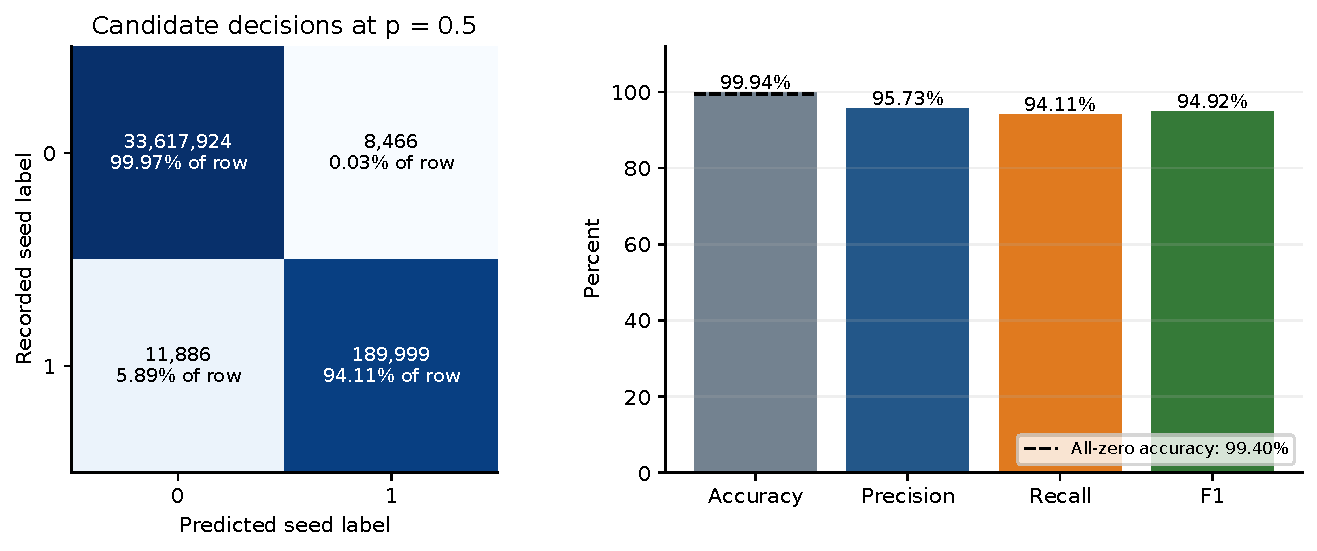
\includegraphics[width=\linewidth]{figures/seed_classification.pdf}
 \caption{Held-out candidate decisions at the fixed probability
 threshold of one half. The matrix gives counts and percentages
 normalized within each reference-label row. The right panel gives
 pooled classification measures. The dashed mark applies only to
 accuracy and shows the result of assigning zero to every candidate.}
 \label{fig:seed-classification}
\end{figure}

The predicted set exactly matched the reference for
@@exact_set@@\% of all test targets. It contained every reference seed
for @@containment@@\% of targets with nonempty reference sets.
These two measures distinguish an identical predicted set from a
larger set that still contains the recorded choice. The fixed model's mean test binary cross-entropy was
@@test_bce@@, with equal weight for each target as in
Eq.~\eqref{eq:seed-training-loss}.

\subsection{Recovering seeds from the ranked candidates}
\label{sec:seed-test-ranking}
The returned probabilities also order the available seeds, which allows
a solver to request further candidates after an initial selection.
For the $k$ highest-ranked candidates, write the selected set as
$\widehat{\mathcal S}_k(\mathcal T)$ and define
\begin{equation}
 R_k(\mathcal T)=
 \frac{\left|\widehat{\mathcal S}_k(\mathcal T)
                  \cap\mathcal S_{\mathcal T}\right|}
      {|\mathcal S_{\mathcal T}|},
 \qquad |\mathcal S_{\mathcal T}|>0 .
 \label{eq:seed-recall}
\end{equation}
The list contains at most $k$ seeds when a family has fewer candidates.
Equal probabilities use the lexicographic order of seed index vectors,
which gives a fixed ordering without reference-label information.

For $k=1,5,10,20$, the target-averaged recall was
@@recall1@@\%, @@recall5@@\%, @@recall10@@\% and @@recall20@@\%,
respectively. The corresponding fractions of targets whose entire
reference sets appeared in those lists were
@@coverage1@@\%, @@coverage5@@\%, @@coverage10@@\% and @@coverage20@@\%.
Figure~\ref{fig:seed-ranked-recovery} also separates individual
integrals from integral expressions, since they can require different
numbers of reference seeds.

\begin{figure}[htbp]
 \centering
 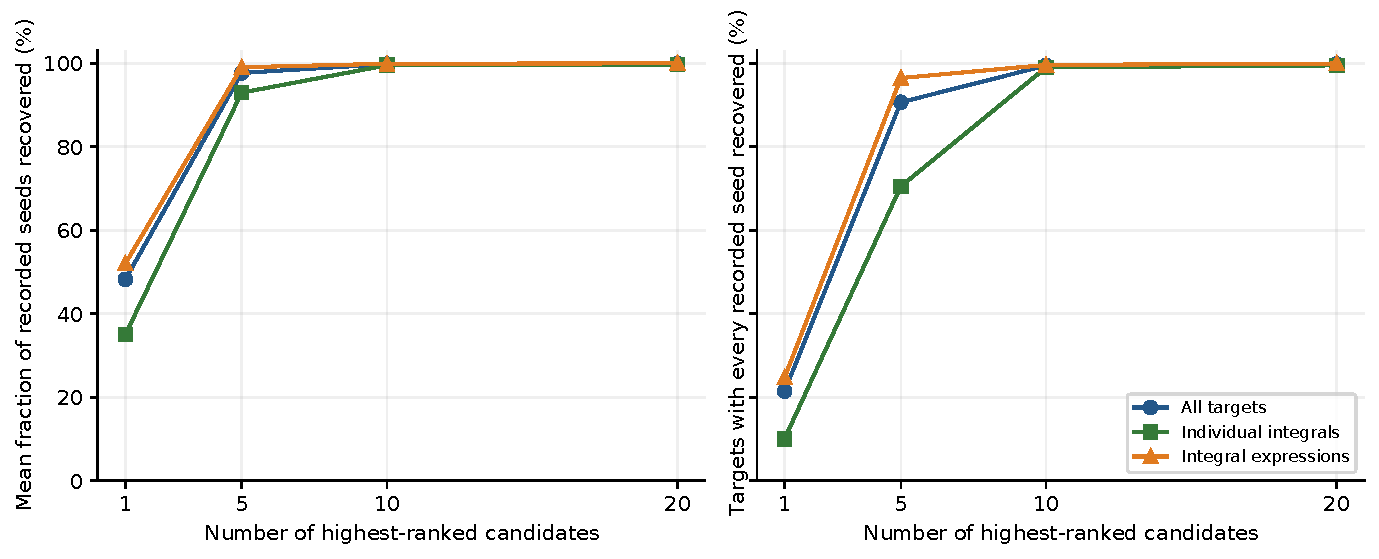
\includegraphics[width=\linewidth]{figures/ranked_seed_recovery.pdf}
 \caption{Recovery from the highest-ranked candidates. The left
 panel averages the fraction of reference seeds recovered per target.
 The right panel gives the fraction of targets whose complete reference
 sets appear in the candidate list. The averages exclude the two
 empty-reference targets. Lines join the four measured candidate counts.}
 \label{fig:seed-ranked-recovery}
\end{figure}

To summarize each target's full ranking, we calculate average precision
over distinct predicted probabilities,
\begin{equation}
 \operatorname{AP}(\mathcal T)=
       \sum_j (R_j-R_{j-1})P_j,\qquad R_0=0 .
 \label{eq:test-average-precision}
\end{equation}
Here $P_j$ and $R_j$ are precision and recall after including every
candidate at the $j$th distinct probability, in descending order.
This definition groups ties and weights precision by the additional
recall at each threshold~\cite{AveragePrecisionDefinition}.
The mean average precision over nonempty targets was @@mean_ap@@,
and its mean over equally weighted family averages was @@family_ap@@.
Figure~\ref{fig:seed-pr} gives the pooled precision--recall curve.
It serves as a diagnostic of the ranking; the reported binary decisions
retain the original threshold.

\begin{figure}[htbp]
 \centering
 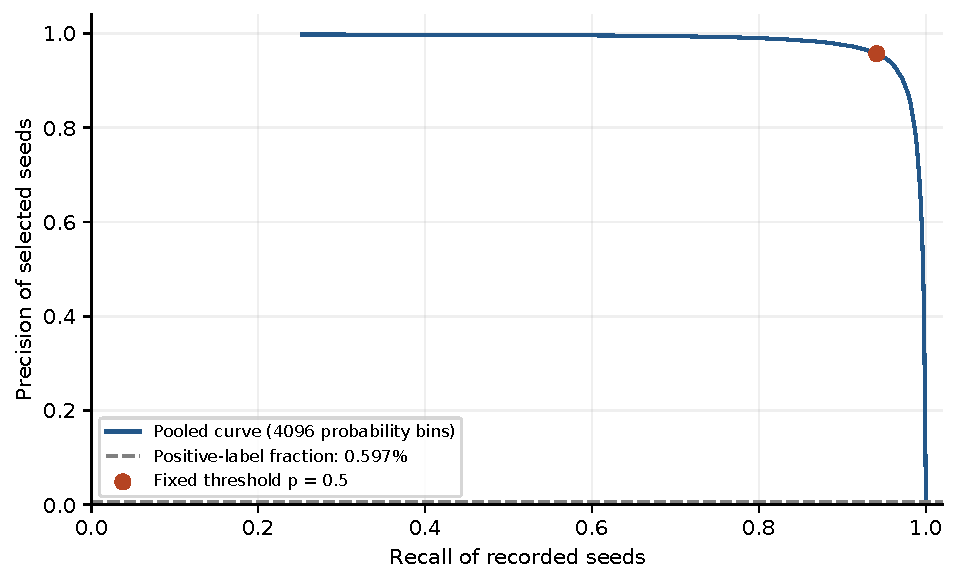
\includegraphics[width=0.82\linewidth]{figures/precision_recall.pdf}
 \caption{Pooled precision and recall across candidate-label
 comparisons. The curve uses 4,096 probability bins to keep memory
 use bounded, so it approximates the continuously varying threshold
 curve. The marked point uses the exact counts at $p_b=1/2$.
 The dashed line gives the positive-label fraction.
 The target average precision reported in the text uses exact
 distinct probabilities, without this binning.}
 \label{fig:seed-pr}
\end{figure}

\FloatBarrier
\subsection{Confidence and variation between integral families}
The confidence $q_b$ in Eq.~\eqref{eq:seed-binary-confidence}
estimates agreement of the returned label with the reference.
We group decisions into intervals of width 0.1 in $q_b$, separately
for returned labels zero and one, and compare mean confidence with
the observed fraction of agreeing labels.
For returned label one, the mean confidence was @@q1@@\% and the
observed agreement was @@q1_agreement@@\%. For returned label zero,
these values were @@q0@@\% and @@q0_agreement@@\%.
Figure~\ref{fig:seed-confidence} displays the populated intervals.
A point on its diagonal has matching mean confidence and observed
agreement. The target-averaged squared probability error was
@@brier@@, where the error for a target is
$n_C^{-1}\sum_b(p_b-y_b)^2$.

\begin{figure}[htbp]
 \centering
 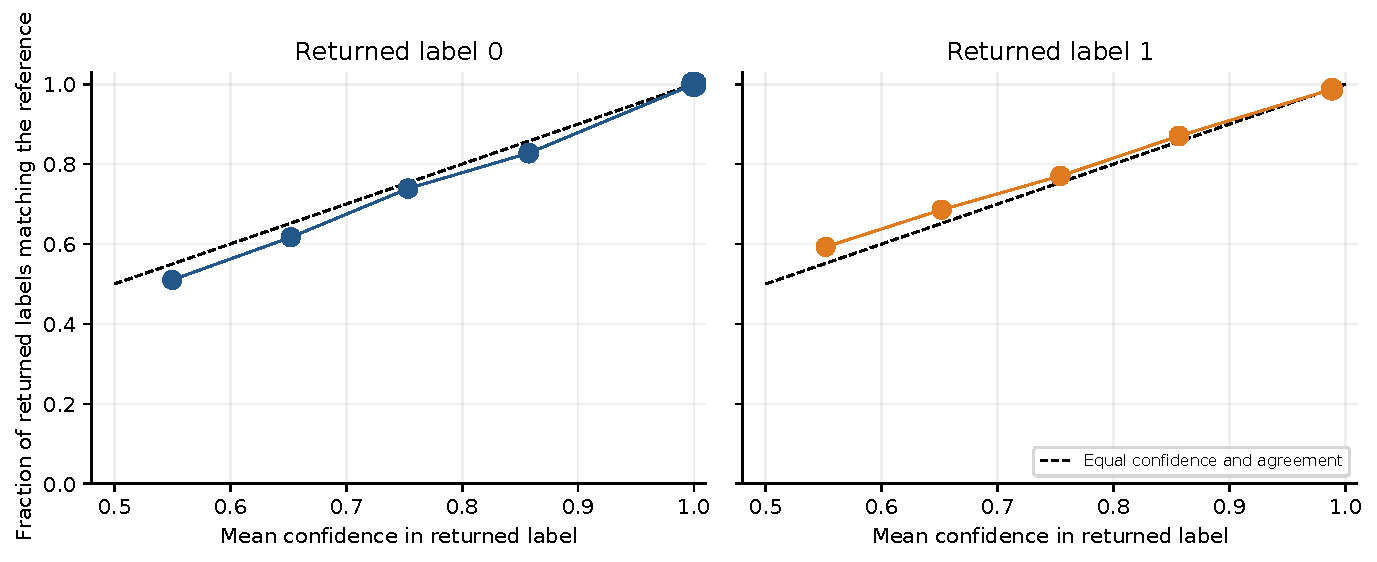
\includegraphics[width=\linewidth]{figures/confidence_calibration.pdf}
 \caption{Confidence in each returned binary label and observed
 agreement with the recorded label. Each point represents one populated
 confidence interval, and larger points represent more candidate
 decisions. The dashed diagonal indicates equal confidence and
 agreement. Separate panels retain the distinction between selected
 seeds and rejected candidates.}
 \label{fig:seed-confidence}
\end{figure}

The pooled precision and recall were @@single_precision@@\% and
@@single_recall@@\% for individual-integral targets, and
@@expression_precision@@\% and @@expression_recall@@\% for integral
expressions. The one-loop group gave @@one_precision@@\% precision
and @@one_recall@@\% recall. @@two_loop_statement@@
Figure~\ref{fig:seed-family-performance} shows the spread of
family-averaged ranking quality and the pooled seed measures at each
loop order. Since the two-loop result comes from one family, it provides
a limited test of transfer beyond the dominant one-loop collection.

\begin{figure}[htbp]
 \centering
 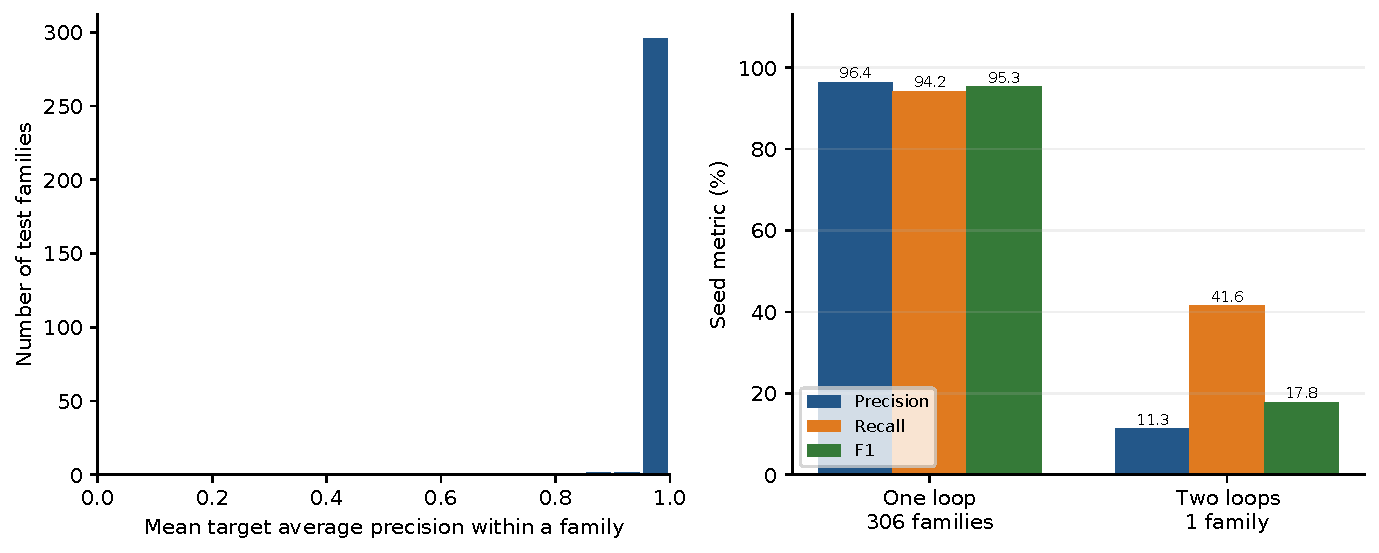
\includegraphics[width=\linewidth]{figures/family_performance.pdf}
 \caption{Variation across the 307 held-out families. The left panel
 gives the distribution of mean target average precision within each
 family. The right panel pools candidate decisions separately for
 306 one-loop families and one two-loop family at the fixed threshold.
 The single two-loop family cannot establish general high-loop
 performance.}
 \label{fig:seed-family-performance}
\end{figure}

\FloatBarrier
\subsection{Implications for IBP reduction}
The test confirms the stated level of agreement with the constructed
reference reductions. The model parameters remained unchanged during
all test calculations. Encoding the target terms and computing their
seed probabilities took a mean of @@input_inference_ms@@ milliseconds
per target on one CPU thread; this timing excludes file reading,
metric calculations and IBP algebra.

The test families are separate from the training families under the
grouping rule in Section~\ref{sec:seed-model-split}. Most of the full
collection shares a one-loop box topology, and lower-sector integrals
can occur in both divisions. The aggregate measures mainly reflect those one-loop examples.
The lower precision and recall of the held-out two-loop family show
that the present model has limited transfer to that family.
The measurements apply to this constructed collection and its bounded
candidate pools.
They do not determine a globally minimal seed set.
A subsequent reduction study must pass the selected seeds to Kira,
check whether their identities reduce each target in the chosen master
basis, and include any extra seeds needed to complete the reduction.
That study will determine the effect on equation counts, memory and
total reduction time.
\FloatBarrier
